\documentclass[../../../../../main.tex]{subfiles}
\begin{document}

\subsection{Overview of the Graphical User Interface}
The GUI will look something like:
\begin{figure}[H]
	\begin{center}
		\includegraphics[width=0.4\textwidth]{diagrams/UI.mps}
	\end{center}
	\caption{UI Design}
\end{figure}
as showcased in the analysis.

Within JavaFX there is a hierarchy\cite{javafxHierarchy} of a standard GUI components. This is shown below:
\begin{figure}[H]
\begin{center}
\begin{forest}
  for tree={
    align=center,
    parent anchor=south,
    child anchor=north,
    font=\sffamily,
    edge={thick, -{Stealth[]}},
    l sep+=10pt,
    edge path={
      \noexpand\path [draw, \forestoption{edge}] (!u.parent anchor) -- +(0,-10pt) -| (.child anchor)\forestoption{edge label};
    },
    if level=0{
      inner xsep=0pt,
      tikz={\draw [thick] (.south east) -- (.south west);}
    }{}
  }
  [Graphical User Interface
    [Stage
      [Scene
        [Node 1]
        [Node 2]
        [Node 3]
        [...]
      ]
    ]
  ]
\end{forest}
\end{center}
\caption{JavaFX Components Hierarchical Diagram}
\end{figure}
\begin{wrapfigure}{r}{0.4\textwidth} 
	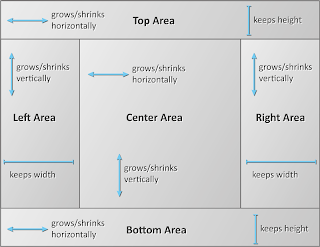
\includegraphics[width=0.4\textwidth]{images/borderpaneArchitecture}
	\caption{Border Pane Architecture}
\end{wrapfigure}
Now we can manipulate the the nodes beneath Scene. It is standard to make the first node beneath Scene some kind of Pane. For this project a Border Pane is most suited since it has regions that can hold sub-nodes. A diagram of this is shown to the right showcases how a Border Pane is arranged\cite{borderpane} and how it behaves.

The center area can consist of the plots themselves, and the left area can consist of the input. The top area could be used for the ribbon and other buttons to manipulate the plot.
\newpage
\end{document}